% A compound move as a tiling of positions 1..n, and the first-tile decomposition
% behind a_n = a_{n-1} + ... + a_{n-k}.
\documentclass[tikz,border=2pt]{standalone}
\usepackage{amsmath}
\usetikzlibrary{arrows.meta}
\begin{document}
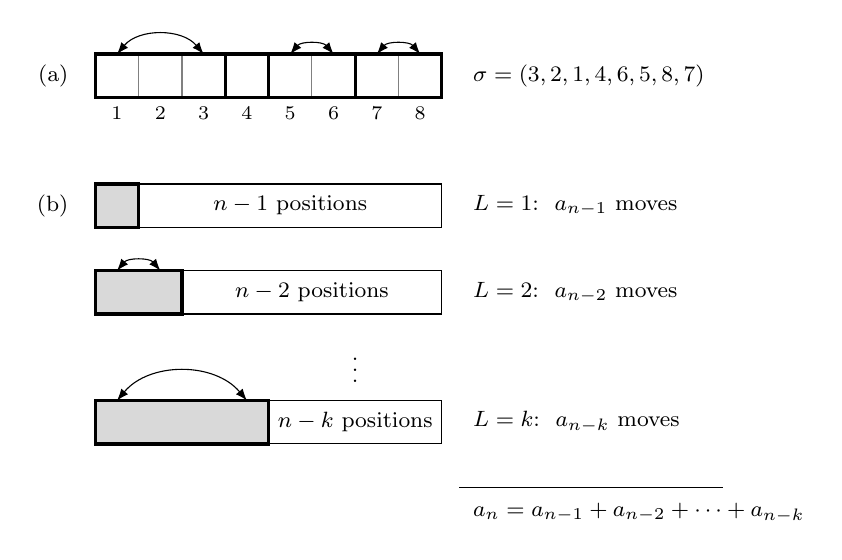
\begin{tikzpicture}[x=0.55cm,y=0.55cm,font=\footnotesize,
  sw/.style={{Latex[length=1.5mm]}-{Latex[length=1.5mm]},bend left=50}]
% (a) the k = 3 move of the board figure: tiles [1,3], [4], [5,6], [7,8]
\node[anchor=east] at (-0.4,0.5) {(a)};
\foreach \t in {1,...,8}{\draw[gray] (\t-1,0) rectangle (\t,1); \node[below] at (\t-0.5,0) {\scriptsize\t};}
\foreach \a/\b in {1/3,4/4,5/6,7/8}{\draw[very thick] (\a-1,0) rectangle (\b,1);}
\foreach \a/\b in {1/3,5/6,7/8}{\draw[sw] (\a-0.5,1) to (\b-0.5,1);}
\node[anchor=west] at (8.5,0.5) {$\sigma=(3,2,1,4,6,5,8,7)$};

% (b) first tile of length L = 1, 2, ..., k; the rest is any move on n - L positions
\node[anchor=east] at (-0.4,-2.5) {(b)};
\foreach \L/\y/\lab in {1/-3/1,2/-5/2,4/-8/k}{%
  \fill[gray!30] (0,\y) rectangle (\L,\y+1);
  \draw[very thick] (0,\y) rectangle (\L,\y+1);
  \draw (\L,\y) rectangle (8,\y+1);
  \node at ({(\L+8)/2},\y+0.5) {$n-\lab$ positions};
  \ifnum\L>1 \draw[sw] (0.5,\y+1) to (\L-0.5,\y+1);\fi
  \node[anchor=west] at (8.5,\y+0.5) {$L=\lab$:\ \ $a_{n-\lab}$ moves};}
\node at (6,-6.1) {$\vdots$};
\node[anchor=west] at (8.5,-9.6) {$a_n=a_{n-1}+a_{n-2}+\dots+a_{n-k}$};
\draw (8.4,-9.0) -- (14.5,-9.0);
\end{tikzpicture}
\end{document}
